\section*{VALIDATION STUDY CASES}\label{sec:validation}
The hybrid method in this paper is investigated using the well known KVLCC2 test case. This ship was selected partly because it is a well known test case and also because it does not have any bilge keels. Ikeda's method contain methods to predict damping from various components, where the bilge keels is one of them. Results from roll decay simulations made with the hybrid method will be compared to corresponding model test data from the SSPA Maritime Dynamics Laboratory. From these model tests, only the total damping can be observed. Reducing the number of components by having no bilge keels will therefore give more insight into the remaining components.

\begin{table}[h]
\small
\caption{KVLCC2 model data}
\label{tab:kvlcc2_model_data}
\begin{tabular}{llllllllll}
\toprule\addlinespacetitle & LPP & B & ZCG & K_{XX} & S & V & \rho & ta & tf\\ 
\midrule & 4.706 & 0.853 & 0.274 & 0.341 & 5.981 & 0.993 & 1000.0 & 0.3059 & 0.3059\\ 
\bottomrule
\end{tabular}
\end{table}
 

\begin{figure}[H]
    \centering
    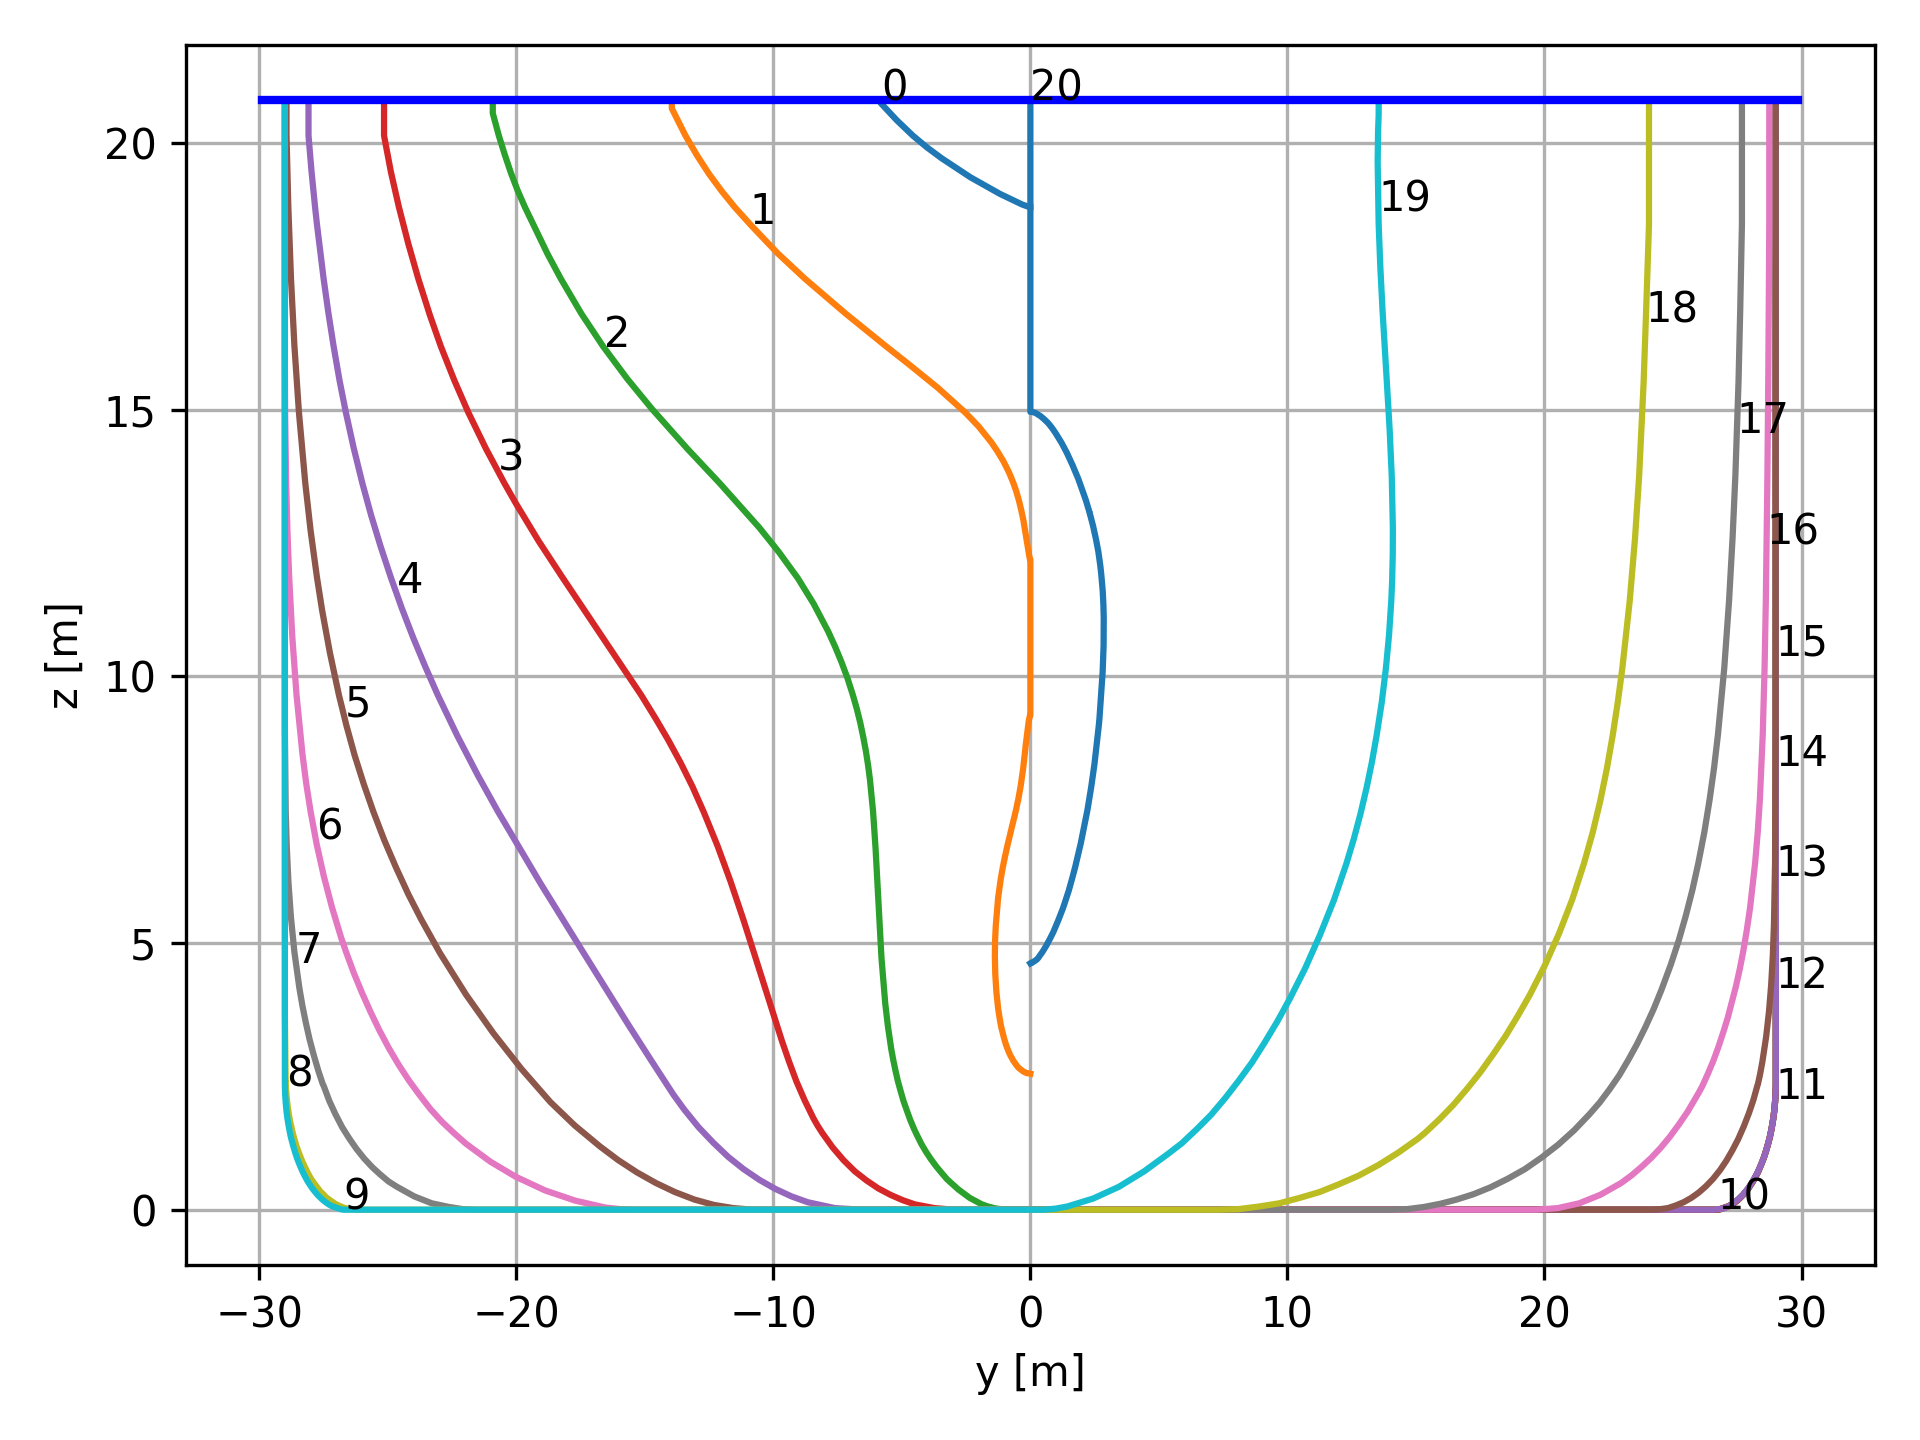
\includegraphics[width = 0.4\textwidth]{figures/body_plan.png}
    \caption{Body plan.}
    \label{fig:body_plan}
\end{figure}            

Revisiting an older semi-empirical method such as Ikeda's method can also be used to gain a deeper understand of the roll damping hydrodynamics.
Time traces of the roll motion from roll decay tests in model scale experiments as well as from FNPF simulations are used in this paper to determine the roll damping of KVLCC2. The PID method is used to identidy the damping from these tests are used: the PIT method.
The $C_r$ was predicted with Ikeda's method and the alternative decision tree model for the KVLCC2 with section data according to the table below. A comparison is shown in the figure below, where it can be seen that the Ikeda implementation predicts much higher $C_r$ between
station 8 and 14, where the bilge radius is also very small.

    \begin{figure}[H]
        \begin{center}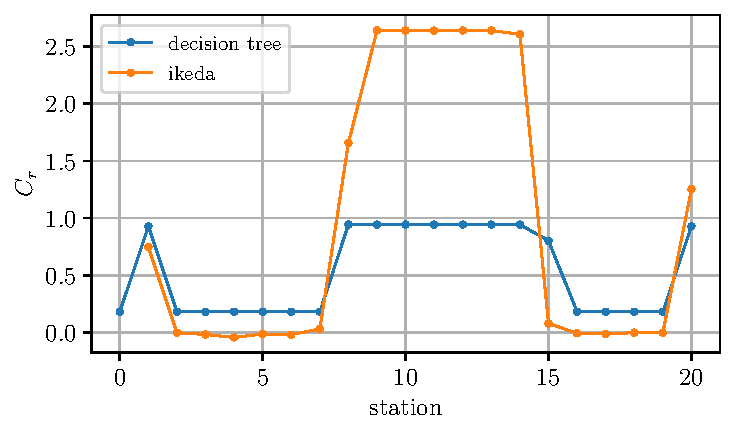
\includegraphics[width = 0.5\textwidth]{figures/kvlcc2_eddy.pdf}\end{center}
        \vspace{-1cm}
        \caption{KVLCC2 eddy}
        \label{fig:kvlcc2_eddy}
    \end{figure}